\documentclass[11pt,titlepage]{article}

\usepackage[american]{babel}
\usepackage[utf8]{inputenc}
\usepackage[T1]{fontenc}
\usepackage{lmodern}
\usepackage{amsmath,amsfonts,amssymb}
\usepackage{graphicx}
\usepackage{geometry}
\geometry{a4paper}
\usepackage[parfill]{parskip}
\usepackage{graphicx}
\usepackage{amssymb}
\usepackage{epstopdf}
\usepackage{stackengine}
\usepackage{color}
\usepackage[tt]{titlepic}
\usepackage{fancyhdr}
\usepackage{enumerate}
\usepackage{lastpage}
\usepackage{float}
\usepackage{amsmath}
\usepackage{amsfonts}
\usepackage{amsthm}
\usepackage{enumerate}
\usepackage{enumitem}
\usepackage{physics}
\usepackage{bm}
\usepackage{setspace}
\usepackage{mathtools}
\usepackage{subcaption}
\usepackage{relsize}
\usepackage{listings}
\usepackage{array}
\usepackage{caption}

% Custom Defines
\usepackage[comma,numbers,sort&compress]{natbib}
\bibliographystyle{plainnat}
\usepackage[pdfstartview=FitH,
            breaklinks=true,
            bookmarksopen=true,
            bookmarksnumbered=true,
            colorlinks=true,
            linkcolor=black,
            citecolor=black
            ]{hyperref}
\newcommand{\rmd}{\textrm{d}}
\newcommand{\bi}[1]{{\ensuremath{\boldsymbol{#1}}}}
\definecolor{gray}{rgb}{0.5,0.5,0.5}

\topmargin=-0.45in
\oddsidemargin=-0.1in
\textwidth=6.8in
\textheight=9.2in
\headheight=30.9pt

\renewcommand{\bibsection}{}
%======================= SET YOUR NAME HERE =======================================
\def\MyName{Matteo Calafà}

%======================= Titlepage (DO NOT MODIFY) ================================
\titlepic{
\includegraphics[width=5cm]{Figures/EPFL_LOGO.jpg}}
\title{\textbf{Report}\\Course Project: Statistics of Turbulence and the Onset of Chaos}

\author{~\\[3cm]~
\begin{tabular}{rl}
Name:&\MyName\\
Date:&\today\\
Course:&Turbulence ME-467\\
Instructor:&Tobias Schneider
\end{tabular}}
\date{}
%==================================================================================



\begin{document}
%========================  Header (DO NOT MODIFY) =================================
\pagestyle{fancy} \pagenumbering{arabic} \setcounter{page}{1}
\addtolength{\headheight}{\baselineskip}
\lhead{\textbf{ME-467: Turbulence}\\\MyName}
\chead{REPORT\\ \textit{Statistics of Turbulence and the Onset of Chaos}}
\rhead{
\includegraphics[width=55pt]{Figures/EPFL_LOGO.jpg}}
\rfoot{\vspace{5pt}{\fontfamily{phv}\fontsize{5}{5}\selectfont ME-467 Project 2022, \MyName{}, \the\day.\the\month.\the\year, \thepage/\pageref{LastPage}}}
\renewcommand{\headrulewidth}{0.4pt}
\maketitle
%==================================================================================

\section{Part I: Statistical Analysis of Turbulence}

\subsection{Introduction} % Remove limit text
This first part regards the classical turbulence theory and a comparison with the results from an experimental setup executed in the Warhaft Wind and Turbulence Tunnel at Cornell University \cite{yoon_warhaft_1990}. In particular, air is driven by a fan that later passes inside the tunnel and downstream velocity is measured by 6 anemometers, each one distant $1m$ from the previous. \\
In this contest, we aim to compare results with both the classical K41 theory and the classical turbulence decay theory. Before starting with the data analysis, it is however important to assure that the experimental setup reflects all the necessary conditions that are fundamental for the theory itself. \\
First of all, since measurements are related to air at an average speed of $10m/s$, we can certainly state that the Reynolds number is sufficiently large to see the effects of turbulence. \\
In addition, homogeneity and isotropy at small scales cannot obviously be fully satisfied in experiments (for instance the collisions with the instruments or the not perfect distribution of velocity at the inlet) but can be reasonably assumed as true in our setup where the inlet from the fan is constant and precise (and, therefore, the forced turbulence is stationary), the direction of the mean flow is approximately horizontal (thanks to the grid between the inlet and the tunnel) and the tunnel is large enough. Moreover, turbulence is fully-developed thanks to the reasonable distance of the anemometers from the inlet.\\
The \emph{finite dissipation rate} for $\nu \rightarrow 0$ is usually assumed as valid in experiments, also because it is a condition that was originally inspired from empirical results (and, indeed, its finite value will be reported in section \ref{the_dissipation_rate_and}). Instead, the \emph{small scale scaling} can be considered true only if the experiment does not show evidence of intermittency, but this fact will be confirmed in section \ref{velocity_signal_in_the_spatial_domain} and \ref{velocity_increments}. \\ 
Moreover, the driving forces (that in this case are represented by the fan action) are evidently applied only on large scales and this will seen later in the energy spectrum analysis (section \ref{energy_spectrum}). \\
As anticipated, the second goal of this part is to analyse in the experiment the characteristics of the turbulence decay under the light of the theory for unforced turbulence. This is the main reason of multiple measurements at different positions that, therefore, should prove a decay in the turbulence quantities because of the absence of applied forces except at the inlet. We will see that the data analysis will be coherent with the theoretical predictions and this means that the conditions of \emph{infrared asymptotic self-similarity} and the \emph{Principle of Permance of Large Eddies} are sufficiently satisfied even in our experimental setup. We also note that our analysis of both the K41 theory (that is for forced stationary turbulence) and the turbulence decay (that is turbulence changing in time) is, as usual, justified by the fact that the power law decay is still very "slow" with respect to the internal turbulence time scales. \\
To conclude this introduction, all the theoretical assumptions are sufficiently satisfied even if, as usual in experiments, some conditions are not completely valid but only approximately (see for instance the $Re\rightarrow \infty$ assumption). This fulfilment will lead to the successful achievement of the theoretical predictions and these laws will be reflected by the experimental results except for inaccuracies that will be justified under the view of measurement imprecisions or the not perfect accomplishment of the above mentioned theoretical assumptions.


\newpage
\subsection{Data Analysis}

\subsubsection{Velocity Signal in the Spatial Domain}\label{velocity_signal_in_the_spatial_domain}
The measurements correspond to streamwise velocities detected at a frequency $f=20kHz$. This implies that each measurement follows the previous one after 
\begin{equation} \label{eq1}
\Delta t = 1/f
\end{equation}
We can exploit the Taylor frozen hypothesis to detect how much two measurements are distant in space knowing the time lag. The distance in space between two following measurements is indeed
\begin{equation} \label{eq2}
	\Delta x \simeq - <u> \Delta t \overset{(\ref{eq1})}{=} -<u>/f
\end{equation}
	where $<u>$ is the mean velocity at each anemometer. Therefore, we can now compute the "virtual" distance in space between two measurements knowing how many measurements there are between them and vice versa: the number of measurements is exactly the ratio of the space distance over $\Delta x$. \\
With this preface, we can execute a first analysis showing in Fig. \ref{fig1} the measurements at each anemometer against the virtual space distance. \\

	\begin{center}
	\begin{figure} [h]
		\centering
		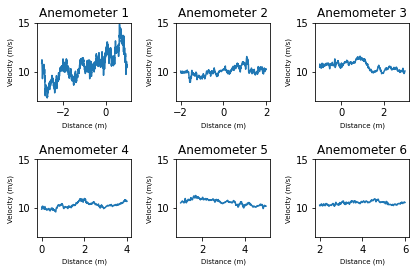
\includegraphics[width = 4.5in]{./figures/ex1_1.png}
		\caption{PLOT A - Streamvise velocity measurements for each anemometer. The plots are shown with respect to space thanks to the Taylor frozen hypothesis.}
		\label{fig1}
	\end{figure}
\end{center}

The $x$ values represent the spatial position of the anemometer and the previous $4m$ as in our choice. First of all, we notice that the mean velocity is almost constant for each anemometer ($\approx 10m/s$). This is expected because of conservation of mass and constant inlet velocity. I.e., the same quantity of air that goes inside the tunnel should goes outside at the same moment if the density is considered constant or almost constant. Because the velocity at the inlet is constant, it implies that the mean velocity should be approximately constant everywhere. \\
On the other hand, oscillations are more evident in the first anemometer and they later vanish. This is expected and due to two main reasons: the first one is the difference between the entrance/unstable region of the tunnel and the fully-developed region where the flow is more asymptotically stable. The second reason is instead related to the decay of unforced turbulence. Clearly, the only applied force is at the inlet of the tunnel where turbulence is therefore more intense. \\
In Table \ref{table1} we instead show the results of mean velocities and turbulence intensities. To obtain them, it is enough to compute respectively the mean and the standard deviation of the velocities measurements at each anemometer, indeed:
\begin{equation*}
	U:=\left<u\right> \hspace{5mm}	I := \frac{\sqrt{\left<\left(u-U\right)^2\right>}}{U}
\end{equation*}

\begin{table} [h]
\centering
\caption{Mean velocity and turbulence intensity} \label{table1}
    \begin{tabular}{ | c | c | c | c | c | c | c | c |}
        \hline
        Param. & Dim. & $A_1$ & $A_2$ & $A_3$ & $A_4$ & $A_5$ & $A_6$ \\
        \hline
        $d$ & $m$ & 1.0 & 2.0 & 3.0 & 4.0 & 5.0 & 6.0 \\
        \hline
        $U$ & $m/s$& 10.522 &10.522& 10.521 &10.522&  10.522&  10.522 \\
        \hline
        $I$ & adim.& 0.1218&  0.0548&  0.0395&0.0320 & 0.0271& 0.0241 \\
        \hline
    \end{tabular}
\end{table}
These results clearly confirm the previous discussion: the mean velocity is almost constant in each anemometer and turbulence intensities instead decrease. Clearly, turbulence intensities are related to the turbulence decay and the decrease of oscillations in Fig. \ref{fig1}. \\
We now notice that Taylor frozen hypothesis is just an approximation of the real phenomenon since turbulence has a certain effect on the flow variations. In general, the approximation is valid if the turbulence intensity is very small but this is not our case (especially at the beginning where this value is more than $0.12$). Moreover, the turbulence intensity changes a lot in space and this gives incoherent results: see for instance in Fig. \ref{fig1} the velocity measurements of the second anemometer at the position $x=-2m$. This trend is completely different from the velocity measured in the first anemometer and associated to the same spatial position. This is because we miss the measurements in the intermediate positions where turbulence intensities have inevitably different values. \\
However, the error in the estimation of intermediate velocity profiles can be easily bounded. The mean velocity is approximately the same in all the positions while the turbulence intensity can be achieved through an extrapolation. In particular, the turbulence intensity follows a trend similar to the ones presented in section \ref{turbulence_decay} (it is indeed equivalent to the square root of the kinetic energy except for a constant coefficient). Therefore, from the results in the table and the assumption of the trend, a regression analysis can be performed to estimate these values in all the intermediate positions. \\
As a last note, we observe from the previous plots that intermittency is not visible and so we assume it to be negligible. Hence, the hypothesis of small scale scaling can still be considered as valid.

\subsubsection{Correlation Length of the Velocity Signal} \label{correlation_length_of_the_velocity}
The autocorrelation function and the integral scale are defined as:
\begin{equation*}
	C(l):=\frac{\left< u(x+l)u(x)\right>}{\left< u^2(x)\right>} \hspace{5mm} L_{int}:= \int_0^\infty C(l) \, dl
\end{equation*}
Moreover, we can approximate $L_{int}$ with the correlation length $L_C$ that is the value for $l$ such that $C(l)$ drops down to $1/e$. \\
In table \ref{tab2} we show the measures of the correlation length and the integral scale. To compute the autocorrelation, we exploited the optimized \texttt{correlate} function from \texttt{Scipy}. To compute the integral scale, we used the same function followed by a rectangular quadrature formula for the integral.  
In Fig. \ref{fig2}, we instead graphically show the trend of the correlation length. \\
\begin{table}[h]
\centering
\caption{Correlation length and integral length} \label{tab2}
    \begin{tabular}{ | c | c | c | c | c | c | c | c |}
    \hline
    Param. & Dim. & $A_1$ & $A_2$ & $A_3$ & $A_4$ & $A_5$ & $A_6$ \\
    \hline
    $L_C$ & m & 0.3667& 0.6345& 0.7733& 0.9039 & 1.0091 &1.0853 \\
    \hline
    $L_\mathrm{int}$ &m &  0.3590& 0.6270& 0.7684& 0.8877 &1.001 & 1.0760\\
    \hline
    \end{tabular}
\end{table}
	\begin{center} 
	\begin{figure} [h]
		\centering
		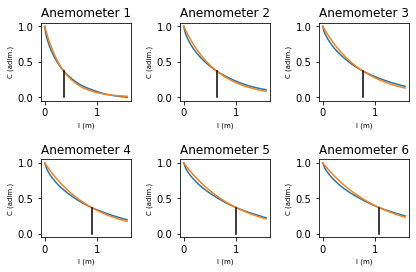
\includegraphics[width = 4.5in]{./figures/ex1_2.png}
		\caption{PLOT B - Correlation lengths with respect to the space distance $l$ (blue curves). Orange lines represent instead the functions $e^{-\frac{l}{L_C}}$. Finally, the black lines are the associated $L_C$ values.}
		\label{fig2}
	\end{figure}
\end{center}
We notice that the two scale lengths are very similar which confirms the fact that the first theoretically approximates the second. Let us clarify this point. Giving a glance at the plots, we recognize soon an exponential decay of the correlation function. Since $C(0)=1$ always (by definition and also from the plots) we conclude that it is approximately in the form: $C(l) = e^{-al}$ for a certain steep coefficient a. It implies that:
\begin{equation*}
	L_{int} := \int_0^{\infty} C(l)\, dl \approx  \int_0^{\infty} e^{-al}\, dl = \frac{1}{a}
\end{equation*}
We now notice that $1/a$ is also the value such that $C(1/a) = e^{-1}$, from here it follows the equivalence of the two definitions of length scale. In addition, these exponential laws are added to Fig. \ref{fig2} to show the effective overlap of the autocorrelation function with its analytical approximation.\\
Let us now discuss the trend of the lengths. Intuitively, we can say that the decaying of turbulence implies a stronger correlation between distant points. In other words, when the turbulence is strong, the noisy dynamics implies the velocity vectors to be almost independent despite they might be close. \\ 
Another reason to convince us of this correct trend is the relation between these length scales and the integral length scale presented in section \ref{energy_spectrum}. We will show later the trend of the latter but we now anticipate that it will increase following the theoretical predictions. Therefore, $L_C$ and $L_{int}$ correctly increase as $l_0$ does.

\subsubsection{Energy Spectrum of the Flow} \label{energy_spectrum}
We define the spectral energy density as $E(k) :=\tilde{E}(k) + \tilde{E}(-k)$ where:
\begin{equation*}
	\tilde{E}(k):= \frac{1}{2} \abs{\frac{1}{\sqrt{2\pi L}} \int_0^L u(x) e^{-ikx}\, dx}^2
\end{equation*}
and $k\in \mathbb{R}$ represents the frequencies and $L$ a maximal measurable distance. 
In Fig. \ref{fig3} we report the measured energy spectrum for each anemometer.
	\begin{center} 
	\begin{figure} [h]
		\centering
		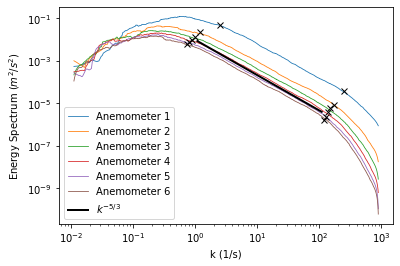
\includegraphics[width = 5in]{./figures/ex1_3.png}
		\caption{PLOT C - Log-log plot of the energy spectrum of the velocity measurements for each anemometer.  Also a black line that indicates the $-5/3$ slope has been inserted.}
		\label{fig3}
	\end{figure}
\end{center}

The energy spectrum has been calculated exploiting the optimized \texttt{fft} algorithm from \texttt{Scipy} for the positive frequencies and the inverse \texttt{ifft} for the negative frequencies. After that, it is just needed to sum the two contributions paying attention to consider the correct multiplicative coefficient (i.e. $(\Delta x)^2$). As a confirmation, we report here the relative error between
\begin{equation*}
	\frac{1}{2}<u^2> \text{ and } \int_0^\infty E(k)\, dk
\end{equation*}
for the first anemometer that turns out to be: $2.47 \cdot 10^{-7}$. These quantities should be theoretically equal because of the Parseval theorem and the relative error is very small because the energy spectrum has been calculated very precisely using the full dataset (this is indeed possible in short times, i.e. less than one minute, thanks to the optimized functions cited above). \\
To conclude the implementation aspects, the original noisy spectrum has been later filtered with a \emph{Savitzky-Golay filter} (\cite{savgol}). More precisely, a standard application of the filter would overshoot in the left part of the plot because, in a log-log plot with originally equidistant $k$ values, the density of the number of points increases towards the right part of the plot. Therefore, a regression-based filter as Savitzky-Golay would be unbalanced in the two different regions. Our proposed solution is to interpolate the original spectrum at points that follow an exponential growth so that, in a log-log plot, they appear equi-distant and the filter can be then well-balanced. \\
We can finally comment the plots in Fig. \ref{fig3} and see how they respect the predictions from the Kolmogorov theory. We can indeed clearly distinguish the three regions (from left to right: the large scales with driving forces, the inertial range and the dissipation region with small scales). In particular, the inertial range clearly respects the $5/3$ law since the straight line is perfectly parallel to the trend of all the anemometers. Moreover, the large scales lines seem to respect the order predicted in the turbulence decay theory (indeed, this will be shown later in section \ref{turbulence_decay}). \\
From the energy spectrum, we can detect the starting and ending points of the inertial range that correspond to the integral and Kolmogorov frequencies. These points have been signed in the plot with black crosses. Finally, from these frequencies, we can get the integral and Kolmogorov length scales that are reported in table \ref{tab3}. \\

\begin{table}[h]
\centering
\caption{Integral and Kolmogorov length scales}\label{tab3}
    \begin{tabular}{ | c | c | c | c | c | c | c | c |}
    \hline
    Param. & Dim. & $A_1$ & $A_2$ & $A_3$ & $A_4$ & $A_5$ & $A_6$ \\
    \hline
    $L_{\mathrm{int},E}$ & m & 2.5133 &5.2360& 6.2832& 6.9813& 7.8540 &8.3776\\
    \hline
    $\eta_E$ & m& 0.0251 &0.0370&0.0419&0.0449& 0.0483& 0.0524 \\
    \hline
    \end{tabular}
\end{table}
Reminding what has been discussed in section \ref{correlation_length_of_the_velocity} about the increase of the correlation length, also here the length scales increase with the distance $d$ because of the same reason as before. \\
As a last result, we want to check effectively the relationship between the two integral scales. This is illustrated in Fig. \ref{fig4}. Here, we show that the two scales are in fact approximately proportional. This fact should not surprise since turbulence length scales are known to be successfully represented by both autocorrelation and spectral length scales and therefore they must scale together (see for instance \cite{trush_2020}).\\
To conclude, we observe that every time $L_{int,E}$ and $\eta_E$ will be used to achieve new results, we will always incur in some inaccuracies due to the graphical detection of these values from the plot that, by its nature, is not precise.
	\begin{center} 
	\begin{figure} [h]
		\centering
		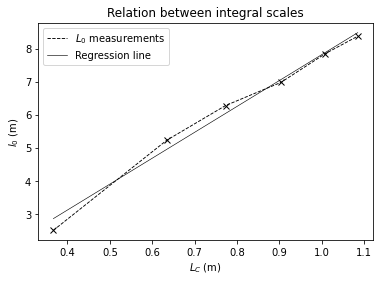
\includegraphics[width = 4in]{./figures/ex1_3_plus.png}
		\caption{EXTRA - Relation between the integral scale length and integral length of section \ref{correlation_length_of_the_velocity}. Despite some inaccuracies due to the rough $L_0$ detection on the plot in Fig. \ref{fig3}, the two values are clearly proportional.}
		\label{fig4}
	\end{figure}
\end{center}


\subsubsection{The Dissipation Rate and Different Reynolds Numbers} \label{the_dissipation_rate_and}
We start by defining the energy dissipation rate and the two Reynolds numbers as:
\begin{equation*}
	\epsilon:=\frac{1}{2} \frac{\sqrt{\left< u^2 \right >^3}}{L_C}, \hspace{5mm} Re_{\lambda} := \frac{\sqrt{\left < u^2\right > } \lambda}{\nu}, \hspace{5mm} Re := \frac{u_0 l_0}{\nu}
\end{equation*}
where $\lambda$ is the Taylor length scale, $\nu$ is the viscosity, $u_0$ is the velocity associated to the large eddies (i.e. the eddies of length $l_0=L_{int,E}$).
In table \ref{tab4} we report these quantities that have been computed starting from the results of the previous sections. \\

\begin{table}[h!]
\centering
\caption{Dissipation rate, Taylor Reynolds and Reynolds numbers} \label{tab4}
    \begin{tabular}{ | c | c | c | c | c | c | c | c |}
        \hline
        Param. & Dim. & $A_1$ & $A_2$ & $A_3$ & $A_4$ & $A_5$ & $A_6$ \\
        \hline
        $\epsilon$ & $m^2/s^3$&2.8708& 0.1511& 0.0466& 0.0211& 0.0116 &0.0075  \\
        \hline
        $Re_\lambda$ & Adim. & 969.5 & 855.4& 802.2 & 780.2& 759.1&
        741.4848821 \\
        \hline
        $Re$& Adim. &$3.10 \cdot 10^5$ & $ 2.91 \cdot 10^5$& $ 2.53 \cdot 10^5$ &$2.28\cdot 10^5$&$ 
        2.18 \cdot 10^5$&$ 2.05\cdot 10^5$ \\
        \hline
    \end{tabular}
\end{table}
We can again give both a physical interpretation and a mathematical explanation to the decreasing trend of $\epsilon$. First of all, as $\epsilon$ represents the rate of turbulent kinetic energy dissipated in thermal energy, it is clear that the decaying turbulence implies a lower rate of energy shift and then a lower dissipation rate for higher $d$. The second motivation is due to the fact that, by definition of $\epsilon$ and the previous relation between length scales, we can state that $\epsilon \sim E^{3/2}/l_0$. Using the rates from the turbulence decay theory (section \ref{turbulence_decay}, equations \ref{l_0_decay}, \ref{E_decay}), we can soon achieve an order of $2h/(1-h)$ for $\epsilon$ with respect to $d$, therefore a power decreasing law. \\
Comparing instead the Reynolds numbers, the decreasing trend is again expected from the theory of turbulence decay and, moreover, $Re_{\lambda}$ scales as the square root of $Re$ (except for a coefficient $\approx 2$) as predicted from K41. \\
To conclude, these trends are all coherent with the turbulence decay results and therefore also with the trend of $I$ from section \ref{velocity_signal_in_the_spatial_domain}.
\subsection{Turbulence Decay} \label{turbulence_decay}
In table \ref{tab5} we report the computations of the kinetic energies per unit mass. This is defined as $\mathcal{E} = 3/2<u^2>$ and the $3$ factor comes from the number of dimensions. Indeed: 
\begin{equation*}
	\mathcal{E} = \frac{1}{2} < \vec{u} \cdot \vec{u} >= \frac{1}{2} < u_x^2 + u_y^2 + u_z^2 > = \frac{3}{2} <u^2>
\end{equation*}
Where the last equality comes from the isotropic assumption. Indeed, what we measure is the streamwise velocity $u_x$ that is assumed to be equal also in the other directions.
\begin{table}[h!]
\centering
\caption{Turbulence kinetic energy per unit mass} \label{tab5}
    \begin{tabular}{ | c | c | c | c | c | c | c | c |}
        \hline
        Param. & Dim. & $A_1$ & $A_2$ & $A_3$ & $A_4$ & $A_5$ & $A_6$ \\
        \hline
        $\mathcal{E}$&$m^2/s^2$ &2.4641& 0.4988& 0.2597& 0.1701 & 0.1223 &0.096  \\
        \hline
    \end{tabular}
\end{table}

We finally report the laws predicted from the theory of turbulence decay:
\begin{equation} \label{l_0_decay}
	l_0 \propto (d-d_0)^{1/(1-h)}
\end{equation}
\begin{equation}\label{u_0_decay}
	u_0 \propto (d-d_0)^{h/(1-h)}
\end{equation}
\begin{equation}\label{Re_decay}
	Re \propto (d-d_0)^{(1+h)/(1-h)}
\end{equation}
\begin{equation}\label{E_decay}
	E \propto (d-d_0)^{2h/(1-h)}
\end{equation}
Where $d_0$ and $h$ are constants. In the next paragraphs, we will equivalently analyse the scaling of $\mathcal{E}$ instead of $E$ (indeed, what changes is the approximately constant mass/density term).
\paragraph{First method:}
The first objective is to find $d_0$ and $h$ from the measurements of $\mathcal{E}$ through a fitting method. Certainly linear regression cannot be used because of the non linearity of the exponent, however we can notice that:
\begin{equation}\label{log_eq}
	\exists K, d_0, b \hspace{3mm} \text{ such that } \hspace{3mm} \mathcal{E}(d) \approx K(d-d_0)^b \hspace{3mm} \Leftrightarrow \hspace{3mm} \ln{\mathcal{E}} \approx \ln{K} + b \ln{(d-d_0)}
\end{equation}
Therefore, applying the logarithm to the data, we only have one non-linear coefficient that is $d_0$. The proposed algorithm is then the following: 
\begin{enumerate}
	\item We iterate over a set of hypothetical values for $d_0$ (numerous enough).
	\item For each of these, we compute the optimal $K$ and $b$ through linear regression.
	\item Given the choice of $d_0,K,b$, we compute the resulting MSE error.
	\item At the end of the loop, we take the $d_0$ that gave the lowest MSE error.
	\item We can finally get the associated $K$ and $b$ again from linear regression.
\end{enumerate}
	This is a simple and quick algorithm since iterations are performed over only one parameter. The resulting values are then: $d_0 \simeq 0.65$, $h \simeq -1.46$. In addition we show in Fig. \ref{fig5} the successful fitting method.
		\begin{center} 
		\begin{figure} [h]
			\centering
			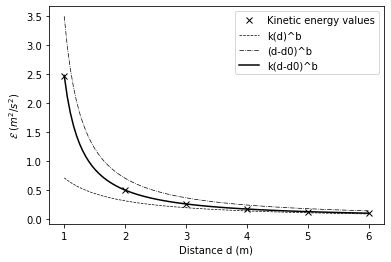
\includegraphics[width = 4in]{./figures/ex1_5_1.png}
			\caption{EXTRA - Fitting of the turbulence kinetic energy per unit mass. The other dashed lines are just to show the importance of both $k$ and $d_0$ parameters.}
			\label{fig5}
		\end{figure}
	\end{center}
	 From now on,  for simplicity, we will consider the optimal exponent as $h=-1.5 = -3/2$. 
	

\paragraph{Second method:}
Taking again equation \ref{log_eq}, we hence have proven that for correct values of $d_0,b,K$ the log-log plot of $\mathcal{E}$ against $d$ is approximately a straight line. Fig. \ref{fig6} shows a  log-log plot of $\mathcal{E}$ against $(d-d_0)$ for different values of $d_0$. For the same reason as before, only the correct $d_0$ generates a straight line. Indeed, only the pink and grey lines are close to be straight, therefore $d_0$ is between 0.6 and 0.7 as confirmed by the fitting method. Taking it in the middle ($=0.65$), we can estimate $q$ looking at the slope of the lines. The black line shows the trend of $\mathcal{E}$ predicted by choosing the previous value for $d_0$ and the correct $q$ to have parallel lines. Looking at the numerical values of $d_0$ and $q$, we conclude that the graphical and fitting methods are coherent. Indeed, for both, the correct shifting parameter is approximately $d_0=0.65$ and the exponent $h=-3/2 \Leftrightarrow q = -6/5$. 

	\begin{center} 
	\begin{figure} [h]
		\centering
		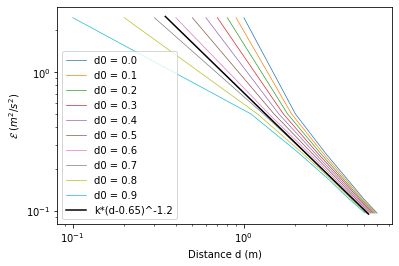
\includegraphics[width = 4in]{./figures/ex1_5_2.png}
		\caption{PLOT D - Log-log plot of the measured $\mathcal{E}$ with respect to $(d-d_0)$ for different $d_0$. As explained in equation \ref{log_eq}, only the correct $d_0$ generates a straight line. Therefore, the correct $d_0$ is between 0.6 and 0.7. Hence, we have chosen $d_0=0.65$.  After that, the exponent $q$ has been chosen such that the line has the same slope. Finally, the graphical method prediction is shown through the black line.}
		\label{fig6}
	\end{figure}
\end{center}


\paragraph{Third method:}
Another confirmation comes from the scaling property:
\begin{equation}\label{eq_E_L0}
	\mathcal{E} \propto l_0^{2h}
\end{equation}
First of all, we inform that we can replace $l_0$ with $L_C$ thanks to the reasons given at the end of section \ref{energy_spectrum}. Therefore, we aim now to study this relation and a comparison between the experimental values of $\mathcal{E}$ against $L_C$ is shown in Fig. \ref{fig7}. 

	\begin{center} 
	\begin{figure} [h!]
		\centering
		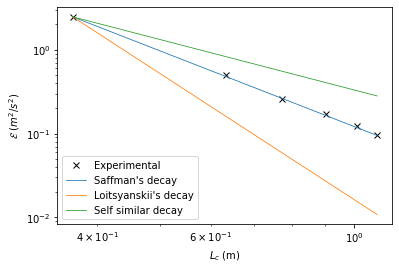
\includegraphics[width = 4in]{./figures/ex1_5_3.png}
		\caption{PLOT E - Log-log plot of the measured $\mathcal{E}$ with respect to $L_C$.}
		\label{fig7}
	\end{figure}
\end{center}

The power law of $\mathcal{E}$ is evident from the straightness of the line. Moreover, these measures coincide almost exactly with the ones from the \emph{Saffman's decay} under which $h=-3/2$. This is expected since we have already shown from the previous methods that $h$ is approximately $-1.5$. \\
Seeing the excellent overlapping of the experimental values with the Saffman's decay predictions, it should not surprise that the fitting method applied  to equation \ref{eq_E_L0} with fixed $h=-1.5$ returns again a parameter $d_0$ that is approximately $0.65$. 

\paragraph{Comparison of the methods:}
To conclude this part about the estimation of $d_0$ and $h$, we can observe that the three methods are indeed equivalent since they return the same values (except for approximations). Advantages and disadvantages of each one are listed below:
\begin{itemize}
	\item The fitting method is very precise. However, it can be a bit slower if compared to the others because of the several calculations (even if it is in general quite fast). In addition, it is harder to interpret results only from the numerical values.
	\item The graphical method is instead good to interpret results. However, it is not precise at all. 
	\item The relation with $L_0$ is precise and has theoretical supports. However, it restricts to only 3 possible theories and it is computationally slow as the first method (since it still needs to iterate over $d_0$).
\end{itemize}

\paragraph{Turbulence decay and energy spectrum: } 
 In Fig. \ref{fig8} we show again the energy spectrum. This time we want to study it with respect to the prediction of its trend for large eddies. Despite some noise (we have already discussed the issue of a fitting/filtering method in a logarithmic scale, see section \ref{energy_spectrum}), the lines seem parallel to the predicted line. Therefore, our theoretical results and the choice of $h=-3/2$ seem to confirm again the experiments.
 
 	\begin{center} 
 	\begin{figure} [h]
 		\centering
 		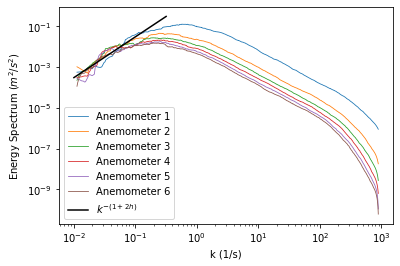
\includegraphics[width = 4in]{./figures/ex1_5_4.png}
 		\caption{PLOT F - Energy spectrum (already shown in Fig. \ref{fig3}) with the theoretical trend for the large scales. Despite some noise, the spectrum seems to scale as the predicted trend.}
 		\label{fig8}
 	\end{figure}
 \end{center}

\paragraph{Discussion about the virtual origin $d_0$:}
The virtual origin $d_0$ is certainly not only a fitting parameter but represents, in a certain way, the starting position for the decaying turbulence predicted trends. In other words, the laws in equations \ref{l_0_decay}, \ref{u_0_decay}, \ref{Re_decay}, \ref{E_decay} do not have any validity for distances $d < d_0$, neither mathematically (exponentials of negative bases) nor physically. Until the distance $d_0$, the turbulence is expected not to freely decay but, instead, to be still forced. This is the reason why our $d_0$ value is between $0m$ and $1m$, i.e. in the inlet region where applied forces have still a dominant role and turbulence is not fully-developed. \\
We expect $d_0$ to be approximately the same for all the above relations (eq. \ref{l_0_decay}, \ref{u_0_decay}, \ref{Re_decay}, \ref{E_decay}) since, the condition of forced/unforced turbulence should hold independently for all the above quantities. Moreover, mathematically, the cited relations are all achieved from one of those and therefore the $d_0$ is the same for each one. However, these are scaling relations and there are inaccuracies in the values achieved for $l_0$ and $Re$, so we do not expect to achieve experimentally the exact same value of $d_0$ for all these quantities. We have indeed performed some fitting methods on equations \ref{l_0_decay} and \ref{Re_decay} fixing the exponent $h=-3/2$ and we achieved respectively $d_0 = 0.75m$ and $d_0 = 0.25m$. Despite these values are not similar with the previous $d_0 = 0.65m$, we still have values in the same interval $0m-1m$ to confirm our theoretical predictions. In addition, we show in Fig. \ref{fig9} that the choice for the $h$ value is suitable also for the $l_0$ and $Re$ values.



\begin{center}
	\begin{figure} [h]
		\centering
		\subfloat[Fitting for $l_0$ values]{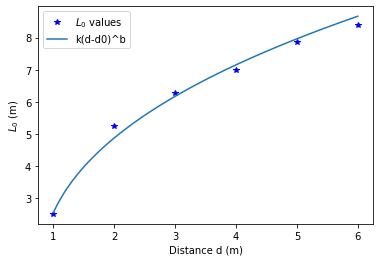
\includegraphics[width = 2.7in]{./figures/ex1_5_5.png}} 
		\hspace{8mm}
		\subfloat[Fitting for $Re$ values]{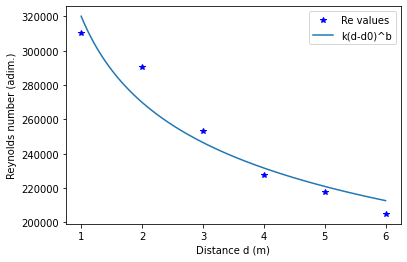
\includegraphics[width = 2.9in]{./figures/ex1_5_6.png}}
		\caption{EXTRA - Fitting method applied to equations \ref{l_0_decay} and \ref{Re_decay} fixing $h=-3/2$. We clearly see that this value for $h$ is well suitable also for these quantities.}
		\label{fig9}
	\end{figure}
\end{center}

\subsubsection{Velocity Increments} \label{velocity_increments}
In Fig. \ref{fig10} we show the behaviour of the longitudinal velocity increment $\delta v_{||}(x,l):=u(x+l)-u(x)$ for the distances $l=\{1mm, 1cm, 10cm, 10m\}$. 
\begin{center}
	\begin{figure} [h]
		\centering
		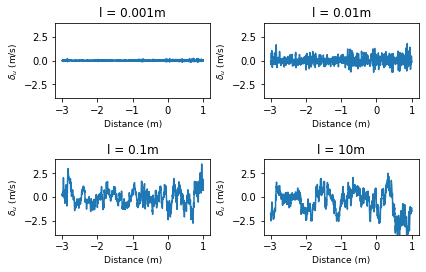
\includegraphics[width = 4in]{./figures/ex1_6.png}
		\caption{PLOT G - Longitudinal velocity increment for different distances $l$ and measured at the first anemometer.}
		\label{fig10}
	\end{figure}
\end{center}

First of all, considering the turbulent length scales in table \ref{tab3}, we can state that:
\begin{itemize}
	\item $l=1mm$ is in the dissipative region ($l<\eta_E$).
	\item $l=0.01m$ is between the dissipative and inertial region ($I \approx \eta_E$).
	\item $l=0.1m$ is in the inertial range ($\eta_E < l < L_{int,E}$).
	\item $l=10m$ is in the large scales region ($l > L_{int,E}$) even if the two lengths are quite comparable.
\end{itemize}

Focusing now on the results from Fig. \ref{fig10}, the behaviour is expected since a small $l$ implies strong similarity between the two measures (that are indeed near in space) where instead a big $l$ implies no connection and therefore a completely random difference. This kind of reasoning is very similar to the one made for the autocorrelation functions in section \ref{correlation_length_of_the_velocity}. In both cases, the increase of distance implies a decrease of correlation. \\
It is important to notice that this increment of randomness has a limit since two measures that are very distant in space are completely uncorrelated and so they show the same pattern whatever is the value of $l\gg0$. As a demonstration, the difference between the case with $l=0.1m$ and $l=10m$ is not so relevant if compared to the upper plots. \\
To further investigate the properties of $\delta u_{||}$ we might wonder whether this has a normal distribution. To do that, we analyse the trend of the flatness that is defined as:
\begin{equation*}
	f(l) := \frac{\left<\delta u_{||}^4(x,l)\right>}{{\left<\delta u_{||}^2(x,l)\right>}^2}
\end{equation*}
For a centred normal distribution, the fourth moment is known to be equal to $3\sigma^4$ while the second moment is the variance. Therefore the flatness is $3\sigma^4/(\sigma^2)^2 = 3$. The flatness of $\delta u_{||}$ is instead shown in Fig. \ref{fig11}.

\begin{center}
	\begin{figure} [h]
		\centering
		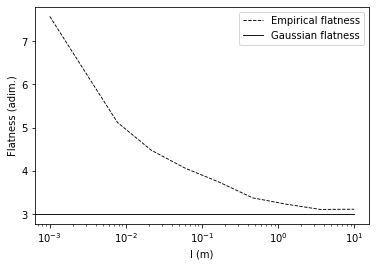
\includegraphics[width = 4in]{./figures/ex1_6_1.png}
		\caption{PLOT H - Longitudinal velocity increment flatness for different $l$. It is easy to see the convergence towards the normal flatness 3.}
		\label{fig11}
	\end{figure}
\end{center}
It is reasonable that the flatness tends to the one from the normal distribution because, as we stated above, big distances imply differences of independent measures and, hence, normally distributed. \\
The reason why the flatness is higher for small distances must be associated to the not normality of $\delta u_{||}(x,l)$ for small $l$. In particular, higher flatnesses are characteristic of the so-called \emph{leptokurtic} distributions, i.e. distributions that are more squeezed at zero and with fatter tails. An equivalent interpretation is the presence of more \emph{outliers}. Therefore, we can reasonably think of $\delta u_{||}$ for small $l$ as more concentrated in zero (see indeed Fig. \ref{fig10}) where, however, there are many outliers due to noisy turbulent effects. Physically, the difference between two near measures is usually small because of the high correlation, however, some noisy sudden effects can sometimes cause completely different measures.

\subsubsection{Structure Functions and Energy Dissipation}\label{structure_functions}
In Fig. \ref{fig12} and  \ref{fig13} we show the trend of $S_2(l)$ and $S_3(l)$ where these quantities are defined as:
\begin{equation*}
	S_n(l):= \left< \delta u_{||}^n(x,l) \right> \hspace{4mm} n \in \mathbb{N}
\end{equation*}
\begin{center}
	\begin{figure} [h]
		\centering
		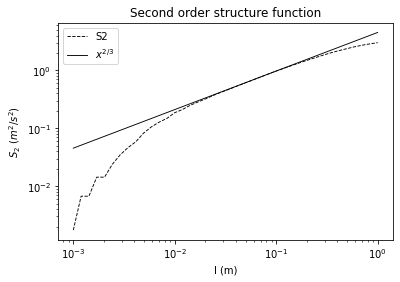
\includegraphics[width = 4in]{./figures/ex1_7_1.png}
		\caption{PLOT I - Second order structure function against distance $l$. In addition, the theoretical trend from K41.}
		\label{fig12}
	\end{figure}
\end{center}
First of all, we note that $S_2$ successfully satisfies the 2/3 law in a certain range. We know from the K41 that the 5/3 law for the energy spectrum is related to the 2/3 law of $S_2$ (more precisely, from the latter we can obtain the former with the Wiener formula). We would like to investigate now whether the 2/3 law has the same range of validity of the 5/3 law in Fig. \ref{fig3}. Since these plots are referred to only the first anemometer, we already computed the Kolmogorov and integral length scale for the first anemometer as $\eta_E \approx 0.025m$ and $L_{int,E} \approx 2.51m$ (table \ref{tab3}). The clear $2/3$ slope is instead observed only in a smaller range: the lower bound is bigger than $0.01m$ and the upper bound is smaller than $1m$. On the other hand, even if this range is shorter, it is centred (not shifted) as the one from the energy spectrum and has more or less the same order of magnitude. \\
\begin{center}
	\begin{figure} [h]
		\centering
		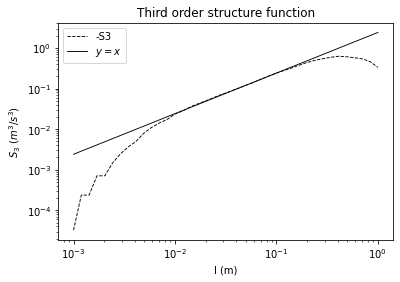
\includegraphics[width = 4in]{./figures/ex1_7_2.png}
		\caption{PLOT J - Third order structure function against distance $l$. In addition, the theoretical trend from K41.}
		\label{fig13}
	\end{figure}
\end{center}
The same could be noticed in Fig. \ref{fig13} for $S_3$ which respects the 4/5 law for a certain range that, also in this case, is similar but shorter than the one from the energy spectrum. To conclude, the trends of $S_2$ and $S_3$ support the K41 except these intervals do not completely correspond to the one from $E(k)$. \\
A last notice is about the fact that from $S_2$ and $S_3$ we could potentially achieve a value for the energy dissipation rate $\epsilon$. Indeed the $2/3$ and $4/5$ laws state that:
\begin{equation} \label{S2_epsilon}
	S_2(l) = C_2 \epsilon^\frac{2}{3} l^\frac{2}{3} \hspace{4mm} \text{and} \hspace{4mm}S_3(l) = C_3 \epsilon l
\end{equation}
where $C_3 = -4/5$ and $C_2$ can be assumed to be $2.2$. Taking a value for $l$ that is valid for these laws (e.g. $l=0.07m$ is in the middle of the validity ranges in Fig. \ref{fig12} and \ref{fig13}) we can then use the inverses of the equations \ref{S2_epsilon} to get $\epsilon$. These values are shown in table \ref{tab6}.

\begin{table}[h]
	\centering
	\caption{Dissipation rate value from $S_2$ and $S_3$ relations} \label{tab6}
	\begin{tabular}{ | c | c | c |}
		\hline
		Method &  $\epsilon$ value ($m^2/s^3$) \\
		\hline
		Standard definition (from table \ref{tab4}) & 2.87 \\
		\hline
		From $S_2$ ($2/3$ law) & 2.97\\
		\hline
		From $S_3$ ($4/5$ law) & 3.01\\
		\hline
	\end{tabular}
\end{table}
These satisfying results confirm again the validity of the theory in our experiment.


\subsection{Discussion} % Remove limit text
In this first part we have comprehensively analysed the dataset from the Warhaft Wind and Turbulence Tunnel to extract important information related to the turbulence behaviour and compared it with the classical K41 theory and the turbulence decay theory. \\
We can conclude that the experiment setup considerably satisfies the assumptions of the theory and indeed all the cited laws have been successfully observed and confirmed by the results. However, the experiment does not lack of outcomes that do not completely fit the theory. Most of these are inevitably due to experimental inaccuracies. For example, one can just think of the detection of the Kolmogorov and integral length scales in section \ref{energy_spectrum}. A graphical method is certainly not precise and, in addition, a different smoothing filter would certainly change the values from the ones predicted here. Moreover, many obtained quantities derive from these length scales or other measurements that are source of error. It is then easy to conclude that experimental imprecisions are as usual omnipresent and inevitable. \\
On the other hand, there are some mismatched results that are probably due to systematic errors. The most relevant example is the range of validity for the $S_2$ and $S_3$ laws in section \ref{structure_functions}. In this case, it would be very interesting to understand if this is due to a not perfect fulfilment of the theoretical assumptions or instead to theoretical laws that are only approximate (i.e. range of validities for the $4/5$ and the $5/3$ laws are known to scale with each other but it is not explicit to which extent and precision). Therefore, we invite further researches to move in this direction. \\
In any case, our experiment successfully confirmed the main theoretical predictions, both in the case of K41 theory of forced turbulence and also for the theory of decaying turbulence. Moreover, all the results that were not directly justified by these theories have been successfully motivated with intuitive, physical and mathematical reasons. To conclude, this experiment fully supports the Saffman's predictions for the turbulence decay.

%==================================================================================
\newpage
\section{Part II: Nonlinear Dynamics and the Emergence of Chaos}


\subsection{Introduction} % Remove limit text
This second part is about the analysis of the dynamics of the generalized Baker's Maps defined as:
\begin{equation} \label{eq_map}
	\begin{gathered}
		x_{n+1} = 
		\begin{cases}
			\alpha_1 x_n & \text{if } y_n < \beta \\
			(1-\alpha_2) + \alpha_2 x_n & \text{if } y_n \ge \beta
		\end{cases}
	\\
	y_{n+1} = 
	\begin{cases}
		y_n/\beta & \text{if } y_n < \beta \\
		(y_n -\beta)/(1-\beta) & \text{if } y_n \ge \beta
	\end{cases}
	\end{gathered}
\end{equation}
where the domain is $[0,1] \cross [0,1]$, $\alpha_1 + \alpha_2\le 1$ and $0<\beta<1$. The visual representation of one step is shown in Fig.  \ref{fig14}.
\begin{center}
	\begin{figure} [h]
		\centering
		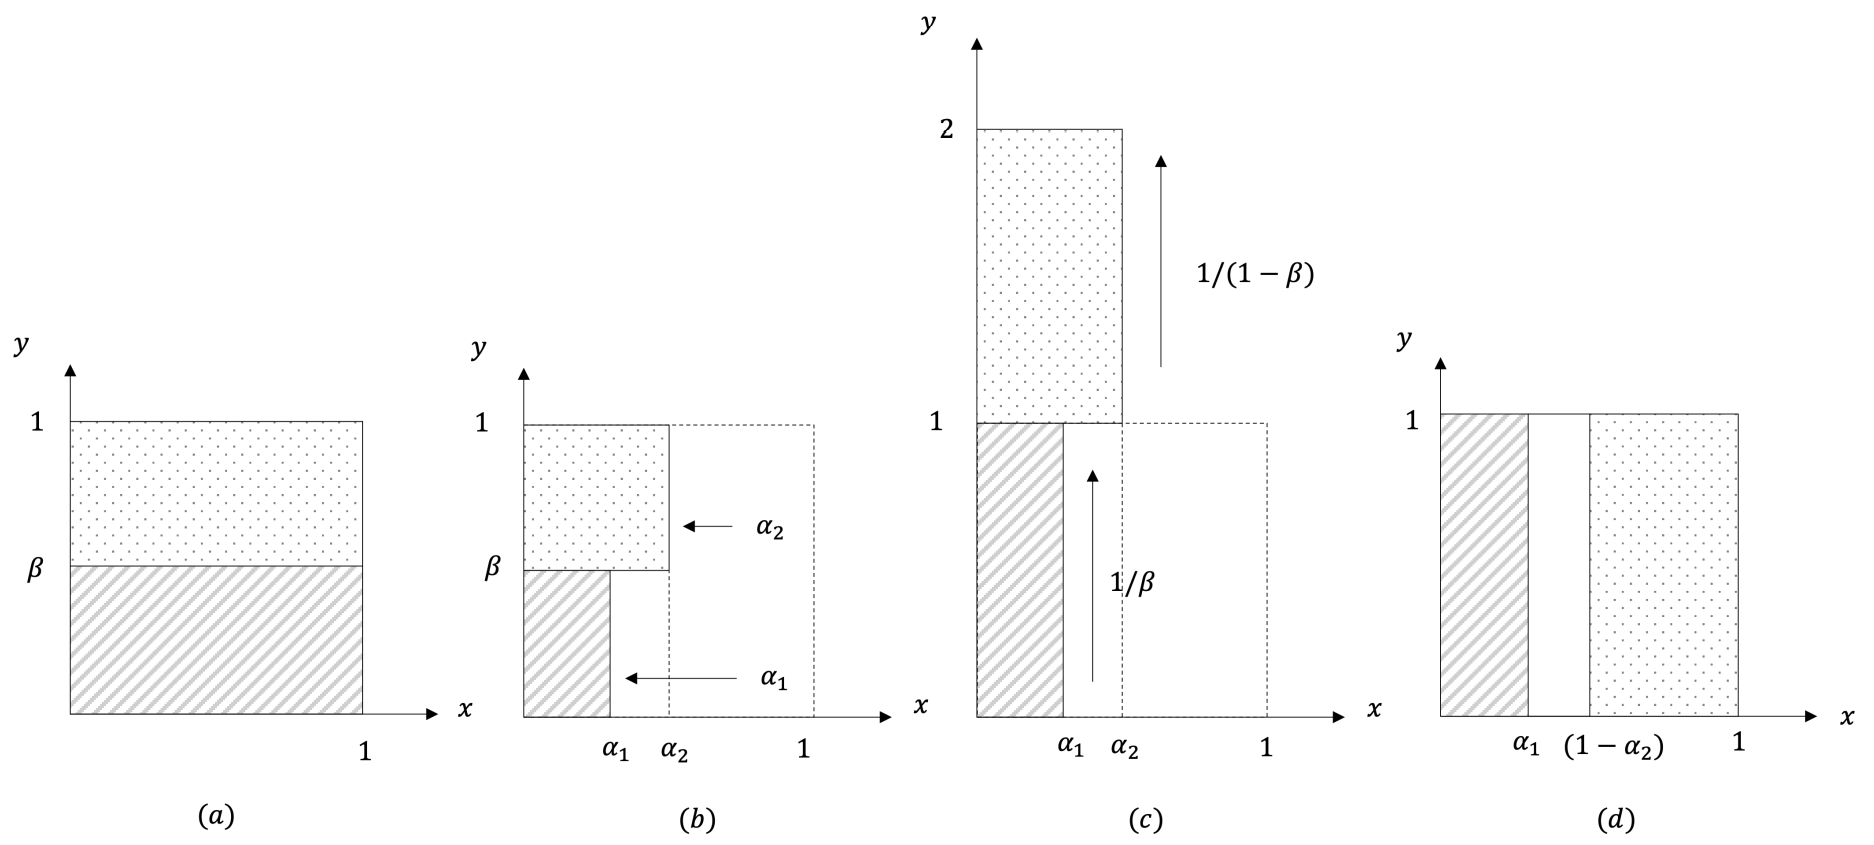
\includegraphics[width = 6in]{./figures/baker_map.png}
		\caption{Graphical representation of the generalized Baker's Map step.}
		\label{fig14}
	\end{figure}
\end{center}
\subsection{Analysis of the Dynamics}
\subsubsection{Implementation of the Map and (Numerical) Observations} \label{implementation_of_the_map_and}
We start by simulating the evolution of this system for some general parameters. A graphical representation is shown in Fig. \ref{fig15}. First of all, thanks to the colour distinction, we recognize soon the equivalence with the dynamics in Fig. \ref{fig14}. At every step, the map firstly separates two regions based on the vertical coordinate. Later, it horizontally shrinks the two regions based on, respectively, the $\alpha_1$ and $\alpha_2$ parameters. After that, it vertically stretches the two regions and, in the end, it places the two new regions at the horizontal borders of the square. Further, what we notice is the continuous addition of new bands that get shorter at every step. The two initial colours, in particular, are separated in all the following bands.
\begin{center}
	\begin{figure} [h]
		\centering
		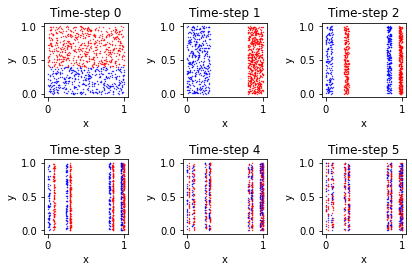
\includegraphics[width = 5in]{./figures/ex3_1.png}
		\caption{Simulated evolution of the map for $\alpha_1=0.3, \alpha_2=0.2, \beta=0.4$. 1000 samples are initialized uniformly in the grid $[0,1]\cross [0,1]$. The blue points are the ones with initial $y_0<\beta$, red points the ones with $y_0\ge\beta$}.
		\label{fig15}
	\end{figure}
\end{center}
Let us now focus on the shape of the attractors for different parameters. These are rectangles that have the full height but a horizontal length that depends on the parameters and the time step. Looking again at Fig. \ref{fig14} we can define explicitly these horizontal coordinates:
\begin{itemize}
	\item For $n=0$: one band from $0$ to $1$.
	\item For $n=1$: two bands from $0$ to $\alpha_1$ and from $1-\alpha_2$ to $1$.
	\item For $n\ge 2$: the same coordinates as in $n-1$ multiplied by $\alpha_1$ plus the same coordinates as in $n-1$ multiplied by $\alpha_2$ and shifted of $1-\alpha_2$.
\end{itemize}
As a confirmation, we have generated the map until step $3$ and drawn the expected bands in Fig. \ref{fig16}. Here, it is evident the above statements are true since all the samples stay inside these borders. \\

\begin{center}
	\begin{figure} [h]
		\centering
		\stackunder[5pt]{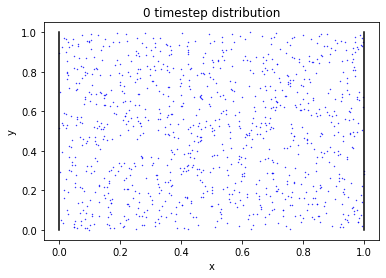
\includegraphics[width = 2.7in]{./figures/quad1.png}}{} 
		\hspace{8mm}
		\stackunder[5pt]{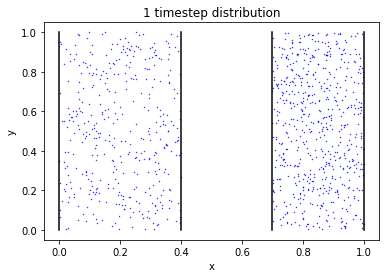
\includegraphics[width = 2.7in]{./figures/quad2.png}}{}
		\\
		\centering
		\stackunder[5pt]{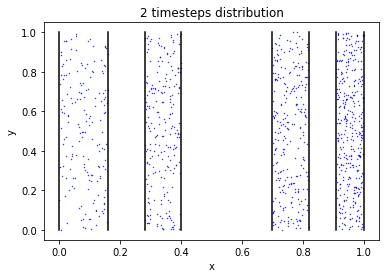
\includegraphics[width = 2.7in]{./figures/quad3.png}}{}
		\hspace{8mm}
		\stackunder[5pt]{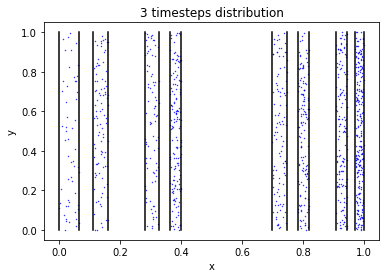
\includegraphics[width = 2.7in]{./figures/quad4.png}}{}
		\caption{Simulated evolution of the generalized Baker's Map (for $\alpha_1=0.4, \alpha_2=0.3, \beta=0.4$, 1000 samples) with the predicted coordinates for the bands.}
		\label{fig16}
	\end{figure}
\end{center}


Now that the general structure of the map has been described, we can analyse the chaotic nature of such system. As a first qualitative description, we take two points that are very close and look at the evolution of  the system for such initial points. Two trajectories of this kind are shown in Fig. \ref{fig17}. Here it is clear that, despite the initial points are very close, eventually the two trajectories split in two different paths. We decided to plot explicitly the Euclidean distance between the trajectories for different parameters. This plot is shown in Fig. \ref{fig18}.

\begin{center}
	\begin{figure} [h]
		\centering
		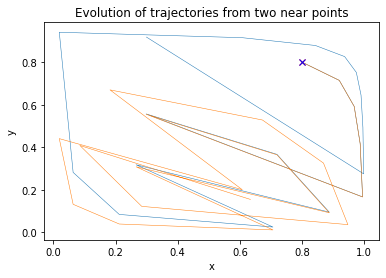
\includegraphics[width = 4in]{./figures/ex3_1_2.png}
		\caption{Simulated evolutions taking two very close points, i.e. $[0.8,0.8]$ and $[0.7999, 0.7999]$ ($\alpha_1=0.3, \alpha_2=0.4, \beta=0.3$). The two points eventually take two independent paths.}
		\label{fig17}
	\end{figure}
\end{center}

\begin{center}
	\begin{figure} [h]
		\centering
		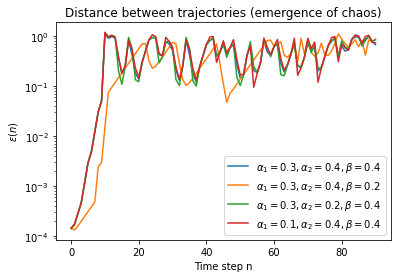
\includegraphics[width = 4in]{./figures/ex3_1_3.png}
		\caption{Euclidean distances between trajectories starting at $[0.8,0.8]$ and $[0.7999, 0.7999]$. Chaos emerges for every choice of parameters. A lower value for $\beta$ seems to reduce a bit the speed of divergence.}
		\label{fig18}
	\end{figure}
\end{center}
To conclude, two near points tend to diverge for every choice of the parameters (except for the special case $\beta=0.5$ as we will see later). Moreover, every trajectory does not convergence and continues to move in different part of the square (as seen in Fig. \ref{fig17}). We can conclude from these qualitative results that the generalized Baker's Map seems to be chaotic. \\
We remind that, in contrast with continuous systems, a 2-dimensional map can potentially be chaotic.


\subsubsection{Strange Attractor and Fractal Dimensions}
In this section, we aim to prove that the map attractors are fractals and we aim to study their characteristics. To do that, we restrict our analysis to the case $\alpha:=\alpha_1=\alpha_2$.  In this case, the bands described in section \ref{implementation_of_the_map_and} have a simpler form since they are completely symmetric. \\
We are going now to compute the \emph{box counting dimension} both analytically and numerically. The idea is to cover the square with a grid composed by many square boxes, then the dimension is defined as:
\begin{equation*}
	D_0 := \lim_{r\rightarrow 0}\frac{\log(1/N(r))}{\log{r}}
\end{equation*}
where $r$ is the length of the little boxes and $N(r)$ is the number of boxes that cover the fractal object. In this case, nothing needs to be done along the $y$ axis that is always all covered. Therefore, we can compute the dimension as $D_0 = 1+D_{0,x}$ where $D_{0,x}$ is the dimension if we consider only the $x$ axis. In addition, it is clear that $\beta$ has no influence in the box counting dimension (bands coordinates depend only on $\alpha$ as we saw before). \\
First of all, let us find a suitable box length for each time step. We aim to get the biggest length such that boxes are aligned with the bands. In this contest, suppose $\alpha \in \mathbb{Q}$, so it is defined by two natural numbers such that $\alpha = a/b$. We can recursively observing that:
\begin{itemize}
	\item $n=0$: the band is in $[0,1]$, therefore one box of length $r=1$ contains all the information.
	\item $n=1$: the bands edges are at the coordinates $\{0, \alpha, 1-\alpha, 1\}=\{0, a/b, (b-a)/b, 1\}$. Therefore, boxes of length $r=1/b$ can be perfectly placed to align the bands ($a$ boxes in the first band, $b-2a$ boxes in the second, $a$ boxes in the last one.)
	\item $n=2$:  the bands edges are at the coordinates $\{0, \alpha^2, (1-\alpha)\alpha, \dots\}$. The same reasoning can be adopted to reveal that $r=1/b^2$ is a divisor of all the coordinates and therefore boxes can be aligned with the bands.
	\item $n\ge 3$: by induction, boxes of size $1/b^n$ are aligned with the bands.
\end{itemize}
Having detected a good value for the box sizes at each step $n$, we know perform the recursive box counting:
\begin{itemize}
	\item $n=0$: one band in $[0,1]$ and one box in $[0,1]$ therefore, trivially, 1 box contains all the points.
	\item $n=1$: there are 2 bands of length $\alpha$. Since boxes and bands of length $1/b$ are aligned, it means that every band contains $\alpha/(1/b) = a$ boxes. Therefore, $2a$ boxes are occupied.
	\item $n=2$: there are 4 bands, each of size $\alpha^2$. Therefore $4 \cdot (\alpha^2 / (1/b)^2) = 4a^2$ boxes are occupied.
	\item $n \ge 3$: by induction, $(2a)^n$ boxes are occupied.
\end{itemize}
We finally have both the box size and the number of occupied boxes for each $n$. The resulting box counting dimension is then:
\begin{equation*}
	D_0 := 1 + \lim_{r\rightarrow 0}\frac{\log(1/N(r))}{\log{r}} = 1 + \lim_{n\rightarrow \infty}\frac{\log(1/(2a)^n)}{\log{(1/b)^n}} = 1 + \frac{\log(2a)}{\log(b)}
\end{equation*}
Let us make some checks with two trivial cases:
 \begin{enumerate}
 	\item If $\alpha=1/2$, the bands correspond to a full cover of the square at each time step (indeed, $\alpha$ coincides with $1-\alpha$). Therefore, the attractive set is the full square at every time step. Not by chance, with $b=2a$ we get $D_0 = 1 + \log(2a)/\log(2a)$ = 2. I.e., the attractive set is not a strange attractor but the normal 2-dimensional square. 
 	\item If $\alpha=1/3$, one can easily see that the limit to the strange attractor along $x$ is the same as the construction of the Cantor set (indeed, it starts with three equally wide bands). In this case, $D_{0,x} = \log(2)/\log(3)$ that is the same dimension of the Cantor set.
 \end{enumerate}
To achieve a numerical result, we simulate the trajectory for $5\cdot 10^6$ uniformly distributed initial points and we use boxes of the size defined above. In particular, we perform the box counting operation for $n=5$. There are other possible choices for $n$ since, from the theory above, for every $n \geq 1 $ we should get the same $D_0$. However, we increase the value $n$ to assure the $\lim_{n\rightarrow \infty}$ operation. On the other hand, bigger values for $n$ would imply smaller boxes and therefore huge memory allocations. This is the reason why we considered $n=5$ as a reasonable value. \\
For the implementation details, it is easy to verify which box the point belongs to using the division of the coordinate over the box length without the remainder. Results are shown in table \ref{tab7}.


\begin{table}[h]
	\centering
	\caption{Analytical and numerical box counting dimensions} \label{tab7}
	\begin{tabular}{ | c | c | c |}
		\hline
		$\alpha$ & Theoretical value & Numerical value \\
		\hline
		$1/5$ & $1 + \frac{\log(2)}{\log(5)} \approx 1.4307$& 1.4307\\
		\hline
		 $1/3$ & $1 + \frac{\log(2)}{\log(3)} \approx 1.631$& 1.631\\
		 \hline
		 $2/5$ & $1 + \frac{\log(4)}{\log5)} \approx 1.861$& 1.824\\
		 \hline
		 $1/2$ & $1 + \frac{\log(2)}{\log(2)} = 2$& 2.000\\
		\hline
	\end{tabular}
\end{table}

As expected, except for $\alpha=2/5$ where some bands are probably not covered by the multiple trajectories, in all the other cases all the bands are correctly covered by points and therefore the numerical solution gives the exact analytical solution. Again, the case $\alpha=1/3$ and $\alpha=1/2$ give the values that are well-known also without the detailed study of the strange attractors.

\subsubsection{Chaos and Lyapunov Exponents}
Other important characteristics of chaotic systems are well described by the Lyapunov exponents. We aim to compute these values analytically and numerically in the case of $\alpha=\alpha_1=\alpha_2$ and $\beta=1/2$ and compare with the behaviour of the system. Consider an initial displacement $\vec{\epsilon_0}$ as we already saw in Fig. \ref{fig18}. Then, the Lyapunov exponent is defined as:
\begin{equation*}
	\lambda := \lim_{n\rightarrow \infty} \lim_{\vec{\epsilon_0} \rightarrow 0 } \frac{1}{n} \log \abs{\left( \prod_{j=0}^{n-1} J_M(\vec{x_j})\right) \frac{\vec{\epsilon_0}}{\abs{\vec{\epsilon_0}}}}
\end{equation*}
where $J_M$ represents the Jacobian of the map. We know that for a $2$-dimensional map there are $2$ Lyapunov exponents and, indeed, the value of $\lambda$ depends on the choice of the displacement direction. \\
Let us firstly compute the Jacobian of the map. A quick analysis to equation \ref{eq_map} with the conditions $\alpha=\alpha_1=\alpha_2$ and $\beta=1/2$ reveals that the partial derivatives are the same in both the cases $y_n < \beta$, $y_n \ge \beta$. Hence, the Jacobian has the following simple form:
\begin{equation*}
	J_M(\vec{x_n}) = \begin{bmatrix} \alpha & 0 \\ 0 & 2\end{bmatrix} \hspace{5mm} \forall n \ge 0 
\end{equation*}
To detect the two exponents, we choose the displacements as parallel to the eigenvectors of $J_M$ that are trivially $\vec{h_1}=[1,0]$ and $\vec{h_2}=[0,1]$ $\forall n\ge0$. Therefore:
\begin{equation*}
	\begin{aligned}
		\lambda_1 = \lim_{n\rightarrow \infty} \frac{1}{n} \log \abs{\begin{bmatrix} \alpha^n & 0 \\ 0 & 2^n\end{bmatrix} \begin{bmatrix} 1 \\ 0\end{bmatrix} } =& \lim_{n\rightarrow \infty} \frac{1}{n} \log (\alpha^n) = \log(\alpha)  < 0 \hspace{4mm} \forall \alpha \le 0.5\\
		\lambda_2 = \lim_{n\rightarrow \infty} \frac{1}{n} \log \abs{\begin{bmatrix} \alpha^n & 0 \\ 0 & 2^n\end{bmatrix} \begin{bmatrix} 0 \\ 1\end{bmatrix} } =& \lim_{n\rightarrow \infty} \frac{1}{n} \log (2^n) = \log(2) \approx 0.693 \\
	\end{aligned}
\end{equation*}
As confirmed by the theory, the Lyapunov exponents are represented by the logarithm of the eigenvalues. These values have also been computed numerically for $n=50$ with different choices for the initial displacement $\epsilon_0$ and $\alpha$. Results are shown in table \ref{tab8}. \\

\begin{table}[h]
	\centering
	\caption{Analytical and numerical Lyapunov exponents for different initial displacements and $\alpha$} \label{tab8}
	\begin{tabular}{ | c |c | c | c |}
		\hline
		$\epsilon_0$ & $\alpha$ & Theoretical $\lambda$ & Numerical value \\
		\hline
		$[0.1,0]$ & 0.4 & $\approx \{ -0.916, 0.693\}$& -0.916\\
		\hline
		$[0.1,0]$ & 0.2 & $\approx \{ -1.609, 0.693\}$& -1.609\\
		\hline
		$[0,0.1]$ & 0.4& $\approx \{ -0.916, 0.693\}$& 0.693\\
		\hline
		$[0,0.1]$ & 0.2& $\approx \{ -1.609, 0.693\}$& 0.693\\
		\hline
		$[0.5,0]$& 0.4 & $\approx \{ -0.916, 0.693\}$& -0.916\\
		\hline
		$[0,0.5]$ & 0.4& $\approx \{ -0.916, 0.693\}$& 0.693\\
		\hline
		$[0.1,0.05]$ & 0.4 & $\approx \{ -0.916, 0.693\}$& 0.677\\
		\hline
		$[0.1,0.05]$& 0.2 & $\approx \{ -1.609, 0.693\}$& 0.677\\
		\hline
	\end{tabular}
\end{table}
Results are expected from the theory. Indeed, every initial displacement that is not parallel to the first eigenvalue generates a limit that tends to be bigger eigenvalue and, hence, to the bigger Lyapunov exponent. In formulae, every $\vec{\epsilon_0}$ that is not proportional to $[1,0]$ returns the second Lyapunov exponent, otherwise the first. \\
Let us see now the relation between these values and the chaotic nature of the system. First of all, as expected, one exponent is positive. Indeed, chaos is generated only if at least one exponent is positive. Not by chance, the positive exponent is the one related to the $y$ direction. It is indeed in this direction that bands are stretched while they are shrunk along the $x$ direction. In addition, if we sum the exponents we get a negative value except for $\alpha=0.5$ that gives zero sum. This should not surprise since, as already seen in Fig. \ref{fig15} and \ref{fig16}, the total area tends to decrease and therefore the system is dissipative. On the contrary, the choice of $\alpha=0.5$ gives the full cover of the square (fractal dimension = 2 as seen before) and hence the area is constant and the system conservative. \\
In the specific case of $\beta=0.5$, the system presents a very singular behaviour that can be well explained by the Lyapunov exponents. First of all, we show in Fig. \ref{fig19} the trend of the displacement in this scenario. \\


\begin{center}
	\begin{figure} [h]
		\centering
		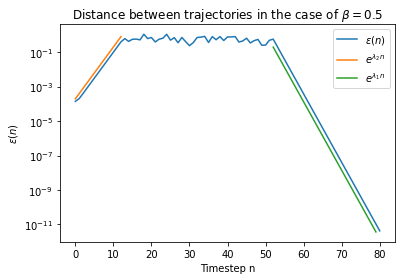
\includegraphics[width = 4in]{./figures/ex3_3.png}
		\caption{Euclidean distances between trajectories starting at $[0.8,0.8]$ and $[0.7999, 0.7999]$ for $\beta=0.5$ and $\alpha=0.4$. Chaos emerges but, after some iterations, the two trajectories come back nearby. In addition, the increase and decrease of distance follow exactly the two Lyapunov exponents.}
		\label{fig19}
	\end{figure}
\end{center}

The fact that the distance initially increases with the same scale of $e^{\lambda_2 n}$  $(\lambda_2=\log(2))$ is clearly expected from the theory but what is not expected is the decrease in the second part. This is observed only in the case $\beta=0.5$ and therefore, it is necessary to look at the law of $y$ more in details. Equation \ref{eq_map} applied to this specific case and only for the $y$ component is the following:
\begin{equation*}
	y_{n+1} = 
	\begin{cases}
		2y_n & \text{if } y_n < 0.5 \\
		2y_n -1 & \text{if } y_n \ge 0.5
	\end{cases}
\end{equation*}
What is observed from the simulations is that $y$ eventually gets the exact 0 value. This is clearly not possible from the theory because the point $(x,y) = [0,0]$ is not a stable equilibrium point. Therefore, this result should be motivated by computational reasons. We know that every number $y \in [0,1]$ is represented by an infinite series of digits $\{I_i\}_{i \in \mathbb{N}}$ such that $I_i \in \{0,1\}$ and:
\begin{equation*}
	y = \sum_{i=1}^\infty \frac{I_i}{2^i}
\end{equation*}
In computer memories, however, this series is not infinite but interrupted at a certain $i=N$. Let us see now the effect of the map on one number with this representation. Hence, we take $y_n$ in this form and distinguish the two cases.
\begin{enumerate}
	\item $y_n < 0.5$: this implies $I_1=0$. Therefore:
	\begin{equation*}
		y_{n+1} = 2y_n = \sum_{i=2}^N \frac{2 I_i}{2^i} = \sum_{i=1}^{N-1} \frac{I_{i+1}}{2^i}
	\end{equation*}
	\item $y_n \ge 0.5$: this implies $I_1=1$. Therefore:
	\begin{equation*}
		y_{n+1} = 2y_n - 1 = 2\left( \frac{1}{2} +\sum_{i=2}^N \frac{I_i}{2^i}\right) - 1 =  \sum_{i=2}^N \frac{2 I_i}{2^i} = \sum_{i=1}^{N-1} \frac{I_{i+1}}{2^i}
	\end{equation*}
\end{enumerate}
Hence, in both the cases, the following value for $y$ has the same representation except one term of the sum less. This means that, if $y_0$ is represented by $N$ digits (this depends on the way memory is allocated), then $y_1$ consists of $N-1$ digits,  $y_2$ is represented by $N-2$ digits until, after $N$ steps, $y_N$ is represented by $0$ digits, i.e. $y_N = 0$. \\
As expected, this is not a result provided by the theory but due to computational reasons. We can now focus on the role of the first Lyapunov exponent. \\
We already know that the system is chaotic because of the positive second Lyapunov exponent that is related to the $y$ direction. However, in this specific case, we know that $y_n$ eventually gets the exact zero value and, so, it will not change its value after the step $N$. This means that our original system transforms to a 1-dimensional system where the $y$ component is fixed to zero. Explicitly, the system becomes:
\begin{equation*}
	\begin{cases}
		x_{n+1} = \alpha x_n \\
		y_{n+1} = 0
	\end{cases}
 	\text{ if } n > N
\end{equation*}
It is now easy to compute the dynamics of the system since we can only focus on $x$.  This means that $\lambda_2$ does not affect the system no more and the only Lyapunov exponent left is $\lambda_1$, that is negative. Therefore, the system cannot be chaotic any more. Indeed, $x=0$ is a stable equilibrium point and we expect trajectories to converge to it. At this point, the speed of convergence is as usual governed by $e^{\lambda_1 n}$ as confirmed in Fig. \ref{fig19}.



\subsection{Discussion} % Remove limit text
In this study we have comprehensively analysed the generalized Baker's map achieving all the main properties. In particular, we have firstly described its geometry and topology for a general choice of parameters underlying the chaotic nature and the fractal structure of the limit attractive set. In the second part we have instead analysed more in details the chaotic behaviour through its Lyapunov exponents. Moreover, we have discussed and motivated the origin of an unexpected result in the specific case $\beta=0.5$ that is not predicted from the theory but originates instead from computational reasons. This last fact should emphasize how computational methods can sometimes be restrictive or even misleading in the study of a dynamical map. In particular, the correct simulation of a Baker's map with $\beta=0.5$ is not trivial. However, in all the other cases, computations have made possible to always achieve numerical confirmations of the theoretical results. Therefore, all the main properties of the map have been analysed and later confirmed.




\clearpage
\appendix
\section*{Appendix}
\subsection*{List of Sources}
\bibliography{sources}
\subsection*{List of Collaborators}
Anna Peruso

%========================  Personal Statement (DO NOT MODIFY) =====================
\subsection*{Personal Statement}
I hereby certify that I fully respect the stated Honor Code and specifically that:
\begin{enumerate}
\item My report is my original work prepared solely by me;
\item All sources used are cited;
\item All people I collaborated with are listed.
\end{enumerate}
		
\vspace{4em}
\begin{tabular}{ll}
\makebox[2.5in]{\hrulefill} & \makebox[2in]{\hrulefill}\\
\small{Signature (\MyName)} & \small{Date}
\end{tabular}
%==================================================================================

\end{document}